\documentclass[a4paper,11pt]{article}
\usepackage[utf8]{inputenc}
\usepackage[T1]{fontenc}
\usepackage[french]{babel}
\usepackage[right=2.5cm, left=2.5cm, bottom=4cm, top=3cm]{geometry}
\usepackage{textcomp}
\usepackage{graphicx}
\usepackage{mathtools,amssymb,amsthm}
\usepackage{lmodern}
\usepackage{multirow}
\usepackage{array}
\usepackage{longtable}

\title{\vspace{13em}{\huge Cahier des Spécifications}}
\author{Edouard Fouassier - Maxime Gonthier - Benjamin Guillot\\
		Laureline Martin - Rémi Navarro - Lydia Rodrigez de la Nava
		\vspace{2em}\\
		Algorithme Génétique
		\vspace{2em}}

\begin{document}
	
	\pagenumbering{gobble}\clearpage
	\maketitle\vspace{13em}
\newpage
\tableofcontents
\newpage\clearpage\pagenumbering{arabic}
	
	\section{Introduction}
		L’algorithme génétique (AG) est un algorithme utilisé principalement pour résoudre des problèmes d’optimisation. 
		Cet algorithme tire son nom de sa particularité à s’inspirer de l’évolution des espèces dans leur cadre naturel.
		Sur le même principe, un AG va faire évoluer une population dans le but d’en améliorer les individus sur plusieurs générations.
		%~De ce fait, à chaque génération c’est un ensemble d’individus qui sera mis en avant et non un seul, représentant un ensemble de solutions au problèmes posé et non une solution unique.
		Les solutions seront généralement différentes mais auront pour particularité de toutes répondre au problème posé.
		%~ Un AG peut également être multicritères, comme par exemple dans le cadre des problèmes d’atelier tel que les Flow Shop ou il convient d’optimiser la minimisation des temps et terminaison mais aussi ceux des retards.

		Un AG peut également dépendre de plus d'un critère, comme par exemple dans le cadre de l'optimisation de la ventilation dans le cas d’un incendie dans un espace confiné où il convient de minimiser la masse de particules aspirées par le système d'aération ainsi que la masse totale de gaz inertant injecté.

		Dans le cadre de notre projet de Semestre 6 de notre licence Informatique, nous devont produire un logiciel utilisant un algorithme génétique dans lequel un utilisateur peut entrer les données de son problème dans une interface graphique et obtenir le résultat de celui-ci en sortie. Le logiciel se doit donc d'être générique pour s'adapter à un maximum de problèmes.
		%~ Afin de pouvoir réaliser une application utilisant un AG pour résoudre des problèmes d’optimisation, nous avons élaboré un organigramme qui en défini la structure. 
		Ce cahier des spécifications regroupe les fonctions, méthodes et classes que nous allons utiliser lors de l’implémentation des différents modules présents dans l'organigramme de notre application qui sera codée dans le langage C++.


	
	\section{Fonctionnement de l'organigramme}
		Voir Organigramme page annexe (page 12)\\

		Lors de l'établissement des spécifications, nous nous sommes vus contraint de changer le découpage de notre organigramme pour qu’il soit en adéquation avec les spécifications de notre application. 
		Avec le découpage initial, nous utilisions uniquement des méthodes de la classe du module "Génération de la nouvelle population" dans les modules "Tests d’arrêt" et "Évaluation de la population", il vaut mieux donc les inclure directement dans le module "Génération de la nouvelle population".
		De même, le module "Gestion de la validité des données" vérifie la validité des données entrées dans un fichier, il peut donc être rapatrié dans le module "Gestion d'entrées sorties". \\
		Toutes ces modifications nous évitent de nous retrouver avec 3 modules artificiels qui n'utilisent que des fonctions et méthodes d'autres modules.
		%~ L’organigramme que nous utilisions initialement n’était pas adapté au développement de notre application et travailler sur le cahier des spécifications de notre projet nous a permis de nous en rendre compte.\\
		%~ Nous avons donc revu l’organisation de notre organigramme p
		%~Les modules "Test d’arrêts" et "Évaluation de la population" sont passés dans le module génération de la nouvelle population. Le module "Gestion de la validité des données" est passé dans le module "Gestion d'entrées sorties".\\

		
		%~ Le module "Interface" de l’organigramme est constitué d’une classe Interface implémentée avec des méthodes de la librairie graphique Qt.\\
		%~ Celui de Gestion des entrées sorties est composé des fonctions utilisées pour valider les données entrées par l’utilisateur dans l’interface, écrire ces données dans un fichier ou bien lire un fichier pour y récupérer les données initiales nécessaires. 
		%~ En plus de cela il permet d’écrire  à chaques itérations la population correspondant à cette itération ainsi que les statistiques qui lui sont associées. 
		%~ Enfin il est également utilisé afin d’écrire les résultats de l’application dans un fichier LaTeX, PostScript ou Xfig.\\
		%~ Le module "Initialisation de la population" est composé uniquement de la classe Individu.\\
		%~ "Génération de la nouvelle population" est composé de la classe Population.
		
		%~ L’organigramme que nous utilisions initialement n’était pas adapté au développement de notre application et travailler sur le cahier des spécification de notre projet nous a permit de nous en rendre compte.\\
		%~ Nous avons donc revu l’organisation de notre organigramme pour qu’il soit en adéquation avec les spécifications de notre application.
		%~ Les modules test d’arrêt et évaluation sont passés dans le module génération de la nouvelle population.
		%~ En effet les tests et l’évaluation on un rapport direct avec la génération d’un nouvelle population, qui correspond à une itération de l’AG, il était donc plus judicieux de rassembler ces trois phases en un seul module .\\
		%~ Le module de validation des données est quant à lui passé dans le module de gestion des entrées sorties puisque les données pour êtres vérifiées doivent être écrites dans un fichier puis lues ensuite.\\
		Dans cette nouvelle version de l’organigramme, l’interface aura pour rôle :
		\begin{itemize}
		\item L’affichage des différents champs de saisie
		\item La réception des valeurs :
			\begin{itemize}
				\item par saisie des champs de l’interface
				\item par fichier
			\end{itemize}
		\item Les options d’arrêt pendant l'exécution de l’application :
			\begin{itemize}
				\item "arrêt" pour arrêter le programme en pleine exécution mais conserver les données
				\item "quitter" pour quitter le programme (perte des données)\\
			\end{itemize}
		\end{itemize}
		Le module de gestion des Entrées Sorties aura pour rôle:
		\begin{itemize}
			\item L’enregistrement des valeurs entrées dans l’interface dans un fichier
			\item La vérification de la validité des valeurs rentrées par l’utilisateur
			\item L’enregistrement des statistiques de l'exécution
			\item L'écriture des résultat en LaTeX/PostScript/Xfig\\
		\end{itemize}
		Le module d’initialisation de la population aura pour rôle:
		\begin{itemize}
				\item La création des individus
				\item L’évaluation des individus\\
		\end{itemize}
		Le module de génération de la nouvelle population aura pour rôle:
		\begin{itemize}
				\item La sélection (par roulette)
				\item Le classement des individus de la population
				\item Le crossover et la mutation
				\item La création de la nouvelle population
				\item La génération de nombres aléatoires\\
		\end{itemize}
		
	\section{Modules}
		Pour faire fonctionner le programme, nous avons besoin de plusieurs choses.\\
		\\

		En premier lieu les données initiales, c'est-à-dire la description du problème de l'utilisateur.\\
		On a besoin tout d’abord de la taille d’un individu. 
		Cette donnée spécifie la valeur maximale que peut prendre une solution, par exemple avec des individus codés en binaire de taille 32, on aura des solutions entre 0 et $2^{32}$ -1.\\
		Il faut aussi le nombre de générations, c’est-à-dire le nombre de populations que l’AG doit créer avant de s’arrêter.\\

		Ensuite, on a besoin de connaître la taille d’une population, c’est-à-dire le nombre d’individus qu’il y a dans une population.\\
		On a besoin aussi de deux probabilités : la probabilité de mutation, c’est-à-dire la probabilité qu’un gène soit modifié, et la probabilité de croisement, c’est-à-dire la probabilité qu’on croise ou pas deux individus. 
		
		On conseille à l’utilisateur de choisir des probabilités petites pour éviter une convergence des résultats prématurée.\\
		On demande aussi à l’utilisateur d’entrer une ou deux fonction fitness.
		Ce sont ces fonctions que l’AG va étudier.
		Chaque fonction fitness est couplée d’un critère, c’est-à-dire qu’on précise si on veut maximiser ou minimiser sur l’intervalle [0, $2^{tailleIndividu}$ -1] ou bien si on veut observer l’évolution de la fonction vers une valeur approchée.
		Enfin, on demande à l’utilisateur d’entrer le nom de fichier de sortie qu’il souhaite, sous forme de chaîne de caractères sans espaces.
		On demande aussi quel(s) format(s) souhaite l’utilisateur.
		Il a le choix entre LaTex, XFig et PostScript, sachant qu’il peut en demander plusieurs.\\
		\\
		Nous avons aussi besoin de plusieurs fichiers :\\

		Un premier qui contient l’ordre des valeurs ainsi que leur type, et qui décrit l'ordre des valeurs dans le fichier de données que l'utilisateur doit suivre s'il souhaite entrer lui-même son fichier de données (exemple : Probabilité de mutation : float). Ce fichier n'est jamais modifié.\\
		Un second dans lequel on enregistre les valeurs initiales que l'utilisateur a entrées. Une fois le valeurs écrites, le fichier n'es plus modifié.\\
		Un troisième dans lequel on écrit tous les scores des individus de chaque génération.\\
		Un quatrième qui contient les statistiques de chage génération.\\

		% Et un dernier qui contiendra la population initiale
		
		\subsection{Interface}
			Pour faire l'interface graphique de notre application, nous avons choisi d'utiliser la librairie Qt car elle est facile à utiliser, générique et donne beaucoup de liberté quand à son utilisation. 
			%~  On peut donner à l’interface l’apparence que l’on veut. 
			%~ e plus Qt s’utilise à la fois sur Windows, linux et mac OS ce qui permet d'envisager un eventuel portage du programme vers ces systèmes.\\

			
			Les includes seront principalement les objets de la librairie Qt 
			(par exemple \#include<QPushButton> pour créer des boutons cliquables).\\
			% mais on aura également le module "Gestion d'entrée sortie" afin d'avoir accès a une fonction.\\
			\\
			\underline{\bf Les attributs privées sont :}\\
				\begin{itemize}
				\item Les objets issus de la librairie utilisés pour l'interface, par exemple :\\
					QPushButton *Lancer : Permet de créer le boutons "Lancer" qui permettra de lancer le programme\vspace{0.2cm}
				\item String fonctionFitness1 : Contient la fonction fitness 1, rentrée par l'utilisateur
				\item String fonctionFitness2 : Contient la fonction fitness 2, rentrée par l'utilisateur
				\item String nomFichierSortie : Contient le nom que l'utilisateur souhaite donner au fichier
				\item int taillePopulation : Contient la taille de la population, rentrée par l'utilisateur
				\item int tailleIndividu : Contient la taille d'un individu, rentrée par l'utilisateur
				\item int nbGenerationMax : Contient le nombre de génération maximum, rentré par l'utilisateur
				\item int critereF1 : 1  = maximisation; 2 = minimisation; 3 = valeur approchée
				\item int critereF2 : 1  = maximisation; 2 = minimisation; 3 = valeur approchée
				\item float tauxMutation : Contient la valeur du taux de mutation rentré par l'utilisateur
				\item float tauxCrossover : Contient la valeur du taux de crossover rentré par l'utilisateur
				\item float valeurApproxF1 : Contient la valeur approché si l'utilisateur a choisi cette option pour la fonction fitness 1, rentré par l'utilisateur
				\item float valeurApproxF2 : Contient la valeur approché si l'utilisateur a choisi cette option pour la fonction fitness 2, rentré par l'utilisateur
				\item bool latex : VRAI si on souhaite que le fichier soit écrit en Latex
				\item bool xFig : VRAI si on souhaite que le fichier soit écrit en XFig
				\item bool postScipt : VRAI si on souhaite que le fichier soit écrit en PostScipt\\
			\end{itemize}

			\underline{\bf Les méthodes publiques slots de la classe sont :}(Ce sont des méthodes qui permettent de connecter des fonction à des éléments graphiques)\\

			\begin{itemize}
				\item \textbf{void connectLancer()} : Lance le programme quand le bouton associé est appuyé. Permet de connecter le bouton "Lancer" et la fonction \textbf{ecrireFichierDonnées(Interface interface, String NomFichier)} du module "Gestion d'entrées sorties".\vspace{0.2cm}
				\item \textbf{void connectQuitter()} : Ouvre une fenêtre de confirmation, puis quitte le programme sans sauvegarder le résultat si confirmé.\vspace{0.2cm}
				\item \textbf{void connectArreter()} : Ouvre une fenêtre de confirmation, puis arrête le programme en sauvegardant le résultat si confirmé. Permet de connecter le bouton "Arrêter" avec la fonction \textbf{ecrireFichier(string nomFichierSortie, string nomFichierParametr, string nomFichier Stats)} du module "Gestion d'entrées sorties".\vspace{0.2cm} 
				\item \textbf{void connectCharger()} : Ouvre le navigateur de fichier pour permettre à l’utilisateur d’indiquer son fichier de paramètre.\vspace{0.2cm}
				\item \textbf{void aide()} : Ouvre le manuel d’utilisation pour aider l’utilisateur.\\
			\end{itemize}
			
			\underline{\bf Les méthodes publiques de la classe sont :}\\\\
			\textbf{Constructeur}
				\begin{itemize}
					\item \textbf{Interface()} : Constructeur par défaut, créant l'interface.\\
					\end{itemize}
			\textbf{Destructeur}
				\begin{itemize}
					\item \textbf{$\sim$Individu()}\\
				\end{itemize}
			\textbf{Getteurs}
				\begin{itemize}
					\item \textbf{String getFontionFitness1()} : Retourne la fonction fitness 1.
					\item \textbf{String getFontionFitness2()} : Retourne la fonction fitness 2.
					\item \textbf{String getNomFichierSortie()} : Retourne le nom du fichier de sortie.
					\item \textbf{int getTaillePopulation()} : Retourne la valeur de la taille de la population.
					\item \textbf{int getTailleIndividu()} : Retourne la valeur de la taille des individus.
					\item \textbf{int getNbGenerationMax()} : Retourne la valeur du nombre de génération maximum.
					\item \textbf{int getCritereF1()} : Retourne la valeur du critère de la fonction fitness 1.
					\item \textbf{int getCritereF2()} : Retourne la valeur du critère de la fonction fitness 2.
					\item \textbf{float getTauxMutation()} : Retourne la valeur du taux de mutation.
					\item \textbf{float getTauxCrossover()} : Retourne la valeur du taux de crossover.
					\item \textbf{float getValeurApproxF1()} : Retourne la valeur approcher de la fonction fitness 1 si il y en a une.
					\item \textbf{float getValeurApproxF2()} : Retourne la valeur approcher de la fonction fitness 2 si il y en a une.
					\item \textbf{bool getLatex()} : Retourne la valeur contenue dans la variable latex.
					\item \textbf{bool getXFig()} : Retourne la valeur contenue dans la variable  xFig.
					\item \textbf{bool getPostScipt()} : Retourne la valeur contenue dans la variable  postScipt.\\
				\end{itemize}
			\textbf{Autre}
				\begin{itemize}
					\item \textbf{void algoGen()} : Lance l'algorithme génétique.
				\end{itemize}
		
		\subsection{Initialisation de la population}
			Ce module est constitué de la classe Individu.\\
			\\
			\underline{\bf Les attributs privés de la classes sont :}\\
				\begin{itemize}
				\item int[tailleIndividu] chromosome : Ce tableau stockera l’ensemble des 0 et 1 qui constituent un individu. C’est ce tableau qui sera évalué pour obtenir le score de l’individu.
				\item int[nombreCritères] score : Ce tableau permettra de stocker le score de l’individu obtenu grâce à la fonction d’évaluation. 
													Dans le cadre d’un problème multicritère il y aura plusieurs fonctions fitness, et donc plusieurs scores par individu.
				\item int[nombreCritères] rang : Ce tableau permet de stocker le rang de l’individu qui sera calculé à partir de son score. 
													Dans le cadre d’un problème multicritère il y aura plusieurs scores, et donc plusieurs rangs par individu. 
				\item static int tailleIndividu : La taille de l’individu sera donnée par l’utilisateur, elle définie le nombre de 0 et de 1 qui composent un individu.
				\item static float probaMutation : La probabilité d’une mutation sur le chromosome d’un individu est donnée par l’utilisateur. Cette probabilité sera utilisée dans la méthode mutation.
				\item static int nombreCritères\\
			\end{itemize}
			\underline{\bf Les methodes publiques de la classes sont :} (On a besoin des méthodes de la classe Individu dans la classe Population, donc on a besoin que celles-ci soient publiques.)\\\\
			\textbf{Constructeurs}
				\begin{itemize}
					\item \textbf{Individu()} : Constructeur par défaut, individu vide
					\item \textbf{Individu (int taille)} : Ce constructeur utilise \textbf{bool probaAlea(float prob)} : Cette fonction renvoie VRAI avec une probabilité flottante prob.
						Il l’applique à tous les gènes jusqu’à ce que l’individu soit complet.
						Cette méthode fait le lien entre le module d’initialisation de la population et celui de génération de la nouvelle population, c'est ce constructeur qui créera un nouvel individu d'une population. 
						En effet pour générer une population il faut créer des individus. \\
								%~ L~a génération d’une population fera donc appel au constructeur de la classe individu pour pouvoir remplir la population.\\
				\end{itemize}
			\textbf{Destructeur}
				\begin{itemize}
					\item \textbf{$\sim$Individu()}\\
				\end{itemize}
			\textbf{Getteurs}
					\begin{itemize}
							\item \textbf{int[tailleIndividu] getChromosome()}
							\item \textbf{int getScore(int i)} : récupère le score à l’indice i
							\item \textbf{int getRang(int i)} : récupère le rang à l’indice i
							\item \textbf{static int getTailleIndividu()}\\
					\end{itemize}
			\textbf{Setteurs}
					\begin{itemize}
							\item \textbf{void ajouterGène(int gène, int i)} : Ajoute un gène (0 ou 1) à l’emplacement i du tableau chromosome.
							\item \textbf{void setChromosome(int [tailleIndividu] chromosome)};
							\item \textbf{void setScore(int score, int i)} : Affecte à l’indice i du tableau de score la valeur score
							\item \textbf{void setRang(int rang, int i)} : Affecte à l’indice i du tableau de rang la valeur rang
							\item \textbf{void setTailleIndividu(int tailleIndividu)};\\
					\end{itemize}
			\textbf{Autres}
				\begin{itemize}
							\item \textbf{Individu codage(int valeur)} : Cette méthode de la classe Individu transforme une valeur entière et la renvoie en binaire sous la forme de tableau d’entier.\vspace{0.2cm}
							\item \textbf{int décodage(Individu I)} : Cette fonction transforme une suite de 0 et de 1 en un entier. Cette fonction sert à obtenir la valeur entière d’un individu.\vspace{0.2cm}
							\item \textbf{bool EvaluationIndividu (String fonctionFitness, int indiceScore)} : Cette fonction prend une fonction fitness et évalue chaque individu en utilisant celle-ci. 
																									Elle prend également un indice correspondant  au score de l’individu afin de pouvoir, dans le cadre d’un problème multicritère, stocker un score par critère. 
																									La valeur obtenue grâce à \textbf{calculfitness(const char *c, double x)} correspondra au score de l’individu et sera écrite dans le tableau des scores à l’indice passé en paramètre.
																									On renvoie VRAI s’il n’y a pas eu de problème lors de l’évaluation, FAUX sinon. Cette fonction est appelée par la méthode Evaluation de la classe Population.
																									Cette méthode fait le lien entre le module d’Initialisation de la population et celui de lGénération de la nouvelle population.
																									En effet pour générer une population il faut en évaluer les individus pour savoir lesquels ont le plus de chance d'être sélectionnés dans la suite de l'algorithme.\vspace{0.2cm}
							\item \textbf{Int mutation(int gene, float prob)} : Cette fonction prend en paramètre un gène, c’est à dire une case du tableau chromosome, et une probabilité.
																		Elle utilise la méthode \textbf{probaAlea(float prob)}, si la méthode renvoie VRAI, alors on modifie le gène et on le renvoie.
																		Sinon, on renvoie le gène sans modification.\vspace{0.2cm}
							\item \textbf{bool probaAlea(float prob)} : Cette fonction renvoie VRAI avec une probabilité prob.\vspace{0.2cm}
							\item \textbf{double calculfitness (const char *c, double x)} : Cette fonction prend la fonction fitness en argument et la valeur de x et renvoie la solution du calcul. La valeur x devra être préalablement transformée en entier par décodage.
								Cette fonction utilisera le parser tinyexpr développé par Lewis Van Winkle. 
								C’est un parser simple et rapide, supportant toutes les formules dont nous avons besoin (racine carré, sin, cos etc…) et facilement adaptable à notre projet. 
								%~ C’est pourquoi nous l’avons choisi.\\
					\end{itemize}
					
		\subsection{Génération de la nouvelle population}
			Ce module est constitué de la classe Population.\\
			\\
			\underline{\bf Les attributs privés de la classes sont :}\\
				\begin{itemize}
				\item static int nombreIndividus
				\item static int nombreCritère
				\item individu[nombreIndividus] ensemble
				\item static int numéroGeneration
				\item static int[nombreCritères] critères : 1  = maximisation; 2 = minimisation; 3 = valeur approchée.
				\item static float valeurApprochée : Si un des critères correspond à une valeur approchée, on stocke la valeur à atteindre ici
				\item static String fitness1 : On limite le problème multicritères à 2 critères
				\item static String fitness2
				\item static int nombreGenerationMax
				\item static float probaCroisement\\
			\end{itemize}


			\underline{\bf Les methodes publiques de la classes sont :} (Dans l'interface qui lancera l’AG on a besoin de la méthode \textbf{creergénération()} et on a ausi besoin de pouvoir évaluer la population, donc on a besoin que les méthodes de Population soient publiques.)\\\\

			\textbf{Constructeurs}
						\begin{itemize}
							\item \textbf{Population()} : Défaut, créer une population sans individu
							\item \textbf{Population(Population p)} : Copie p dans la population créée
							\item \textbf{Population(String nomFichierDonnées)} : Crée une population avec les données initiales et utilise le constructeur de la classe Individu pour remplir la population de manière aléatoire\\
						\end{itemize}
			\textbf{Destructeur}
					\begin{itemize}
							\item \textbf{$\sim$Population()}\\
					\end{itemize}
			\textbf{Getteurs}
					\begin{itemize}
							\item \textbf{int getNombresIndividus()}
							\item \textbf{individu[nombreIndividus] getEnsemble()}
							\item \textbf{int getnumeroGeneration()}
							\item \textbf{String getFitness1()}
							\item \textbf{String getFitness2()}
							\item \textbf{float getValeurApprochée()}\\
					\end{itemize}
			\textbf{Setteurs}
					\begin{itemize}
							\item \textbf{void setNombresIndividus (int nombre individu)}
							\item \textbf{individu[nombreIndividus] setEnsemble()} : Cette fonction ajoute un individu à l’indice i dans l’ensemble de la population.
																			Elle doit vérifier que la population n’est pas pleine.
							\item \textbf{void setnumeroGeneration (int numeroGeneration)}
							\item \textbf{void setFitness1(String fitness1)}
							\item \textbf{void setFitness2(String fitness2)}
							\item \textbf{void setValeurApprochée(float valeurApprochee)}
							\item \textbf{void setProbaCroisement(float probaCroisement)}
							\item \textbf{void setNombreGenerationMax (int nombreGenerationMax)}\\
					\end{itemize}
			\textbf{Tests}
				\begin{itemize}
							\item \textbf{Population TestArret()} :  Cette fonction teste si on doit continuer à itérer l’algorithme génétique ou non. 
								On teste l’arrêt avec les deux fonctions ci-dessous. 
								Si les deux fonctions renvoient VRAI, on continue l’itération de l’AG et on envoie la population au module de Gestion d’entrées/sorties pour qu’il écrive les scores dans le fichier. 
								Sinon on arrête l'algorithme et la population est envoyée au module de gestion d’entrées/sorties pour écrire le fichier final.\vspace{0.2cm}
								\begin{itemize}
								\item \textbf{bool TestNombreGénération()} : Cette fonction teste si on a atteint le nombre d’itérations que souhaite l’utilisateur.
									Elle renvoie VRAI si la valeur n’est pas atteinte, FAUX sinon.\vspace{0.2cm}
								\item \textbf{bool TestConvergence()} : Cette fonction vérifie que les dernières populations ne convergent pas, c'est-à-dire que les valeurs n'évoluent plus. %Il utilise static int numéro$\_$generation pour retrouver les générations qu'il doit étudier.	
								Elle utilise le fichier où sont écrites les statistiques de toutes les générations. Elle va lire en particulier les moyennes réduites des 10 générations précédentes
															%~ TestConvergence renvoie VRAI si une des deux conditions suivantes est remplie.
															%~ Sinon il renvoie FAUX.Dans un premier temps il vérifie les critères.
															%~  Si parmis les critères il y a la recherche d’une valeur approchée alors il lit cette valeur entrée par l'utilisateur.
															%~ Il va comparer cette valeur avec la moyenne réduite des scores de la population actuelle.
															%~ Si les deux sont identiques (+/- 1,5$\%$), il renvoie VRAI.Ensuite on va lire les moyennes réduites des 10 générations précédente et la comparer avec celle de la population actuelle.
															Si plus de quatre moyennes réduites consécutives sont égale(+/- 1,5$\%$) à celle de la population actuelle, on renvoie VRAI.

															Si le critère est de trouver une valeur approchée, alors on compare uniquement la moyenne réduite de la population actuelle et la compare à la valeur entrée par l'utilisateur.\vspace{0.2cm}
								\end{itemize}
							
							\item \textbf{Bool TestPopRemplie()} : Cette fonction teste la taille de la population. Si la population est remplie, c’est-à-dire si sa taille est la taille maximum d’une population, elle renvoie VRAI, sinon FAUX.\vspace{0.2cm}
					
					\end{itemize}
				
			\textbf{Autres}
				\begin{itemize}
							\item \textbf{Population Evaluation()} : Cette fonction sert à donner un rang à chaque individu pour faciliter la sélection. 
								Elle appelle EvaluationIndividu puis PopulationTri pour pouvoir se servir du score des individus et établir un classement. 
								Elle ne prend pas de paramètre puisque toutes les données nécessaires sont des attributs de la classe population. 
								Elle renvoie une population où chaque individu se sera vu attribuer un rang en fonction des critères à évaluer (maximisation, minimisation ou obtention d’une valeur approchée).\vspace{0.2cm}
								\begin{itemize}
								\item \textbf{bool TriPopulation (int indiceScore)} : Cette fonction prend un indice afin de savoir à quel score se référer. 
									Elle permet de trier les individus de la population dans l’ordre croissant de leur score.\vspace{0.2cm}
								\end{itemize}
							
							\item \textbf{Individu Sélectionner()} : Cette fonction sélectionne un individu parmi la population et le renvoie. 
								Elle utilise l’algorithme de sélection par roulette décrit dans le cahier des charges.\vspace{0.2cm}
								
							\item \textbf{Population crossover(Individu Parent1, Individu Parent2, float prob)} : Cette fonction prend deux individus choisis par la fonction \textbf{Sélectionner()}, les croise pour en créer deux nouveaux qui seront ajoutés à la population puis on renvoie celle-ci. 
							Si la prob décide que deux individus ne sont pas croisés, cela veut dire qu’on ajoute directement ces deux individus dans la nouvelle population. 
								Elle utilise la fonction \textbf{nombreAlea(int inf, int sup)} pour déterminer le point de croisement, pour pouvoir créer les nouveaux individus en croisant les moitiés des deux individus.
								Avant de copier les gènes dans les nouveaux individus, on les entre un par un dans la fonction \textbf{mutation(int gène, float prob)}. 
								Les deux nouveaux individus sont ajoutés directement dans la population  avec la fonction addIndividu.\vspace{0.2cm}
							
							\item \textbf{Population créerGénération(Population P)} : Cette fonction crée une nouvelle population à partir d’une population P.
								Tout d’abord, elle crée une nouvelle population vide grâce au constructeur de la classe. 
								Ensuite, elle utilise la fonction \textbf{crossover(Individu Parent1, Individu Parent2)} pour créer deux nouveaux individus et les ajouter dans la population qu’on vient de créer.
								On continue d’utiliser le crossover jusqu’à ce que la nouvelle population soit pleine.\vspace{0.2cm}
							
							\item \textbf{Int nombreAlea(int inf, int sup)} : Cette fonction sélectionne aléatoirement un entier entre inf et sup.

					\end{itemize}
			
		\subsection{Gestion d'entrées sorties}
			Ce module constitue la partie procédurale du programme.\\
			\\
			\underline{\bf Pour la validation}, on utilisera les methodes suivantes :\\
			\begin{itemize}
				\item \textbf{bool testCoherenceDonnéees (String nomFichier)} : C’est la fonction qui s’occupe de tester les valeurs entrées par l’utilisateur en vérifiant que chaque donnée correspond bien au type qu’elle est censée avoir, si l'utilisateur décide d'entrer son propre fichier de données. Cette fonction n'est pas utilisée si l'utilisateur entre ses données via l'interface.
					Elle prend en entrée le nom du fichier où sont écrites les valeurs et renvoie VRAI si l'écriture s'est bien passée.
					Pour vérifier le type, on a un fichier où sont écrits pour chaque donnée son nom et le type qu’elle doit avoir.\\
					Elle utilise les 5 fonctions qui suivent. On souhaite que le programme puisse entrer dans les fonctions même si les valeurs ne sont pas du bon type, donc les paramètres sont auto.\vspace{0.2cm}
				\item \textbf{bool estEntierPositif (auto valeur)} : Cette fonction prend une valeur et renvoie VRAI si la valeur est un entier positif FAUX sinon.\vspace{0.2cm}
				\item \textbf{bool estFloatPositif (auto valeur)} : Cette fonction prend une valeur et renvoie VRAI si la valeur est un nombre flottant positif FAUX sinon.\vspace{0.2cm}
				\item \textbf{bool estProbabilité (auto valeur)} : Cette fonction prend une valeur et renvoie VRAI si la valeur est un nombre flottant entre 0 et 1, FAUX sinon.\vspace{0.2cm}
				\item \textbf{bool estString (auto nom)} : 	Cette fonction prend une valeur et renvoie VRAI si la valeur est une chaîne de caractère, FAUX sinon.\vspace{0.2cm}
				\item \textbf{bool estParsable (String fonction)} : Cette fonction prend une chaîne de caractère qui correspond à la fonction fitness et renvoie VRAI si la fonction est correcte, FAUX sinon. On dira qu’une fonction est correcte si elle a uniquement 1 variable qui devra toujours être noté x, s’il n’y a pas de division par 0, si elle est correctement parenthésée et si les opérateurs binaires ont bien une opérande de part et d’autre. De plus on vérifie que les fonctions supportées soit bien orthographiés : log, sin, cos, sqrt, pow, exp, log10, tan et fac.  Un exemple de fonction fitness pourrait être : cos(x)+4*x-5. On doit utiliser cette fonction aussi dans le module Interface.\\
			\end{itemize}
			
			\underline{\bf Pour la lecture}, on utilisera les methodes suivantes :\\
			\begin{itemize}
				\item \textbf{int[3] lireStats (File* F )} : Cette fonction prend en entrée le fichier où se trouvent les statistiques d’exécution de l’algorithme et renvoie un tableau de taille 3 contenant la moyenne, le minimum et le maximum des scores de la ligne où se trouve le pointeur F. Elle sera utilisée pour résumer le déroulement de l'AG dans le fichier final.\vspace{0.2cm}
				\item \textbf{float[3] lireInfoRegen(String nomFichier)} : lis le fichier des DI et renvoie un tableau comportant en 0 le taux de crossover et en 1 le taille de la population, en 3 le nombre de critères.
					Cette fonction fait le lien entre le module de gestion des Entrées Sorties et celui de génération de la nouvelle population.
					Elle permet de lire dans le fichier de données les valeurs nécessaires à la création d’une population.\vspace{0.2cm}
				\item \textbf{float[3] lireInitialisation (String nomFichier)} : lis le fichier des DI et renvoie un tableau comportant en 0 nombre de critère, en 1 la taille d’un individu et en 2 le taux de mutation.Cette fonction fait le lien entre le module de gestion des Entrées Sorties et celui d’initialisation de la population. 
					Elle permet de lire dans le fichier de données les valeurs nécessaires à la création d’un individu.\vspace{0.2cm}

				\item \textbf{int lireScoreIndividu(String nomFichierPopulation, int gén, int i)} : Cette fonction lit à le i-ème individu de la génération gén dans le fichier qui contient tous les scores, et renvoie sa valeur. Elle sera utilisée notamment pour calculer les statistiques.\\

			\end{itemize}
			
			\underline{\bf Pour l'écriture}, on utilisera les méthodes suivantes :\\
			\begin{itemize}
				\item \textbf{bool ecrireFichierDonnées(Interface interface, String NomFichier)} : Cette fonction écrit dans le fichier Interface.nomFichier les données entrées dans l’interface par l’utilisateur. 
					C’est l’interface qui fournit à la fonction le nom du fichier où les données doivent être écrites, et un tableau qui contient les données dans l’ordre qu’on a choisi. 
					Elle renvoie FAUX s’il y a une erreur lors de l’écriture, VRAI sinon.\\
					Cette fonction permet de faire le lien entre le module de l’Interface et celui de gestion des Entrées Sorties en prenant les valeurs entrées par l’utilisateur en paramètre ainsi qu’un nom de fichier prédéfini afin de créer un fichier qui stocke les données.\vspace{0.2cm}
				\item \textbf{bool ecrirePopulation (Population P, String nomFichier)} : Cette fonction prend comme argument une population et le nom d’un fichier. 
					Elle se charge d’écrire les scores de chaque individu de la population P dans le fichier nomFichier. 
					Elle sera appelée à chaque création d’une nouvelle population. %, il faut donc aussi écrire de quelle itération de l’algorithme il s’agit, valeur qu’on trouve dans la classe Population.\\
					Cette fonction permet de faire le lien entre le module de génération de la nouvelle population et celui de gestion des Entrées Sorties. 
					Elle prend en paramètre une population ainsi que le nom du fichier contenant les résultats de l’application et écrit la population dans le fichier. 
					Cela permet de garder une trace de toute l’éxécution de l’application et d’analyser les données.\vspace{0.2cm}
				\item \textbf{bool calculerEcrireStats(Population P, String nomFichierPopulation, String nomFichierStats)} : Cette fonction cherche le score minimum, maximum,la moyenne de tous les scores et la moyenne réduite des scores. 
					Pour cela elle lit dans le fichier où se trouvent les scores, fait les calculs, puis écrit les résultats dans le fichier des statistiques. 
					Elle récupère le score d’un individu avec \textbf{int lireScoreIndividu(String nomFichierPopulation, int génération, int indice)}. %qui renvoie le score de l’individu situé à l’indice i de la génération passée en argument dans le fichier nomFichierPopulation.
					%cette fonction correspond à la fonctionnalité du calcul des statistiques qui sservent ) décrire l’évolution de l’algorithme dans le fichier de sortie de l’utilisateur.
					%Pour la moyenne réduite des score on veut savoir combien d'extrêmes il faut enlever.
					%Ainsi on fait : (static int nombre$\_$individus) / 5 si c'est pair et (static int nombre$\_$individus - 1) / 5 si c'est impair.
					Cette fonction permet de faire le lien entre le module de génération de la nouvelle population et celui de gestion des Entrées Sorties. 
					Elle permet de stocker les statistiques de chaque génération dans un fichier afin de les exploiter ensuite dans la réalisation d’un graphique.\vspace{0.2cm}
				\item \textbf{bool ecrireFichier(string nomFichierSortie, string nomFichierParametre, string nomFichier Stats)} : Cette fonction teste quel type de sortie l’utilisateur désire puis fait appel aux 3 fonctions ci-dessous. 
					Elle utilise le fichier des paramètres et le nom du fichier des statistiques pour la création du fichier final. 
					Chacune des fonctions renvoie FAUX s’il y a une erreur dans l’écriture. Elles utilisent la fonction lireStats pour remplir le fichier de sortie.\vspace{0.2cm}
				\item \textbf{bool ecrireLatex(string nomFichierSortie)} : Cette fonction crée un fichier NomFichierSortie.tex.
					Elle renvoie FAUX s’il y a une erreur lors de l’écriture, VRAI sinon.\vspace{0.2cm}
				\item \textbf{bool ecrirePostscript(string nomFichierSortie)}  : Cette fonction crée un fichier nomFichierSortie.ps.
					Elle renvoie FAUX s’il y a une erreur lors de l’écriture, VRAI sinon.\vspace{0.2cm}
				\item \textbf{bool écrireXfig(string nomFichierSortie)}  : Cette fonction crée un fichier nomFichierSortie.xfig.
					Elle renvoie FAUX s’il y a une erreur lors de l’écriture, VRAI sinon.\vspace{0.2cm}
				\item \textbf{bool écrireUnScore(int score, FILE *F)} : écrit un score à l’emplacement du pointeur F.
					Elle renvoie FAUX s’il y a une erreur lors de l’écriture, VRAI sinon. \\
			\end{itemize}
		
		\subsection{Notions du langage utilisées}
			L’utilisation du C++ pour le développement de notre application nous permet d’utiliser des notions propres aux langages orientés objets.
			En premier lieu la notion d’objet, en effet l’interface est dans notre application un objet identifiable.
			Nous utilisons également des méthodes pour décrire le comportement des objets que nous utilisons.
			Les individus et les populations qui seront instanciés durant l'exécution de notre application sont également des objets sous forme de classes puisque ce seront deux ensembles d’objets ayant tous le même type dont le comportement sera dicté par les mêmes méthodes.
			Les attributs de ces deux classes étant privés nous utilisons aussi la notion d’encapsulation afin de ne pas pouvoir modifier d’attributs par inadvertance.
			La classe population devra durant le déroulement de l’application communiquer avec la classe individu, nous profitons donc de la notion d’envoi de message pour communiquer entre plusieurs objets.
			La notion de surcharge est utilisée, notamment pour les constructeurs des classes Individu et Population.
			La notion d’héritage n’est en revanche pas utilisée puisque les classes Individu et Population n’ont pas le même comportement, il n’est pas utile de créer un lien d’héritage entre les deux.
			Le polymorphisme, la lésion tardive des méthodes et la génériques ne sont en revanche pas utilisé dans notre application.\\

	
	\section{Conclusion}	
		Nous avons explicité dans ce cahier des spécifications le contenu de chaque module pour répondre aux problèmes décrits dans le cahier des charges.
		Nous y avons notamment décrit les types et propriétés des attributs et méthodes de nos classes.
		Nous avons désormais un schéma clair et précis de notre futur logiciel, ce qui nous assurera une implémentation sûre et un partage des tâches optimisé.
		
	\newpage
	\section{Annexe}
		\subsection{Organigramme}
		\centerline{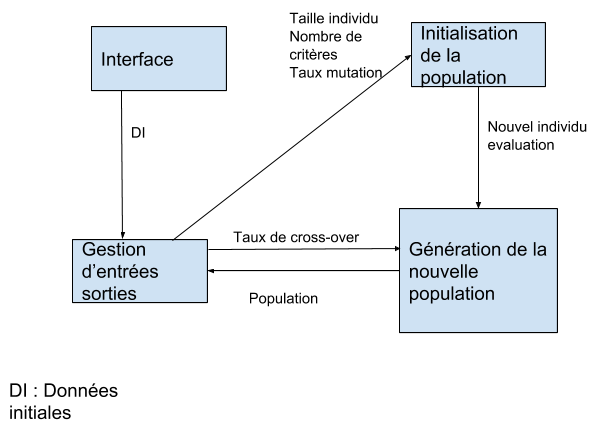
\includegraphics{OrganigrammeV7.png}}
		
		\subsection{Apercu de l'interface}
		\centerline{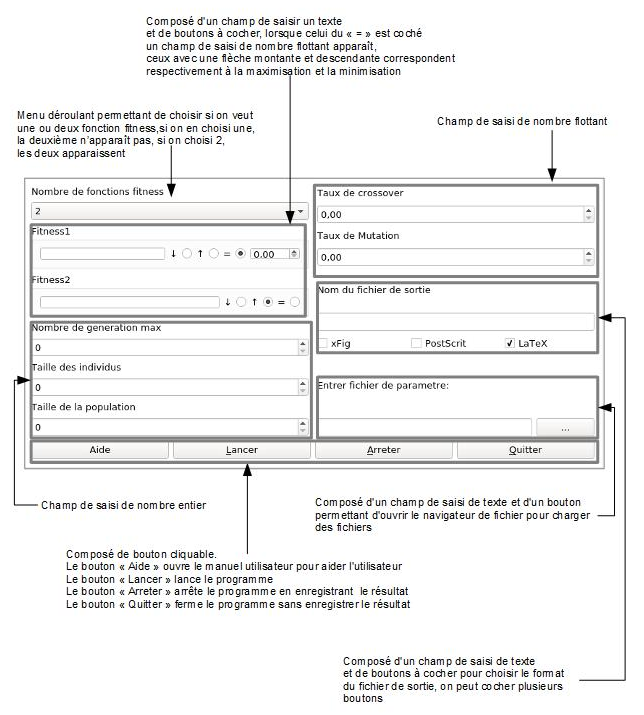
\includegraphics{InterfaceExpliquer.png}}
	
\end{document}
